\rhead{METHODOLOGIES ET PROCEDURES}

\lettrine[lines=2,slope=0pt,nindent=4pt]{\textbf{A}} chaque type d'action, un processus spécifique est défini afin que celle-ci soit traitée au mieux. On dénombre 4 types différents d'action : développement, étude, demande de maintenance (ayant elle-même plusieurs catégories) et livraison. \\
Chacune a sa propre méthodologie de traitement qui est spécifiée dans cette partie. Le responsable de l'action doit suivre cette méthodologie afin de garantir sa qualité de réalisation et éviter d'oublier certaines étapes cruciales.

\chapter{\label{chapter:dev}Processus de d\'eveloppement}
\lhead{Processus de d\'eveloppement}
\rhead{METHODOLOGIES ET PROCEDURES}
Un développement consiste à introduire un nouveau modèle, une nouvelle fonctionnalité ou nouvel outil dans le code. Le respect d'une méthode de développement (ou bonnes pratiques) a plusieurs avantages :
\begin{itemize}[label=$\Rightarrow$, font=\LARGE]
   \item Elle permet de réduire considérable la dette technique du code. Les coûts ultérieurs, tant pour la maintenance corrective (correction de bugs informatiques) que pour la maintenance évolutive (mise à jour ou ajout de fonctionnalités) peuvent être plus ou moins importants selon la mise en oeuvre de ces bonnes pratiques. Ces coûts additionnels représentent la dette technique d'un logiciel. Une méthodologie de développement permet ainsi de maîtriser les temps de développement mais aussi de réduire la fréquence des bugs.
   \item Elle permet d'accroître la sécurité du logiciel.
   \item Elle permet d'obtenir un code ayant en permanence une bonne qualité jusqu'au moment où une opération de valorisation est envisagée (préparation des audits).
   \item L'application de bonnes pratiques rend propoice le travail en collaboration en établissant un "code de conduite" commun à tous les acteurs.
\end{itemize}

La méthodologie de développement appliquée à TrioCFD va donc être explicitée dans ce chapitre.
\subsection{\label{subsec:specif}Étape 1 : Sp\'ecifications}
Cette étape d'expression du besoin doit être faite en tout premier lieu par le développeur en charge de l'action. Elle doit couvrir l'intégralité des cas d'utilisation du code, en expliquant ce qui doit être fait et non pas comment le faire. Chaque spécification doit pouvoir être testée lors de la dernière phase du développement.
Pendant cette phase de spécification, le développeur doit :
\begin{itemize}[label=$\Rightarrow$, font=\LARGE]
   \item identifier les besoins puis les traduire en termes de fonctionnalités, d'interfaces avec les autres Baltiks de TrioCFD, avec TRUST, avec les autres Baltiks de TRUST mais également entre elles ;
   \item préciser les enchaînements des actions ;
   \item préciser les contraintes liées au développement (performances, priorités,...) ;
   \item analyser, en fonction des besoins à couvrir, les classes ou Baltiks qui pourraient être réutilisés et évaluer les impacts de leur réutilisation sur le développement.
\end{itemize}

Ces spécifications fonctionnelles doivent s'affranchir de la façon dont est implémentée le code. Il est important de les établir pour ne pas se lancer aveuglément dans le codage. \newpage
Lors de cette étape, il est pertinent de faire une analyse bibliographique des différents modèles à disposition pour arriver au besoin ciblé. Par cette analyse bibliographique, les avantages et inconvénients des différents modèles pouvant répondre au besoin seront identifiés, de même que leur adéquation avec la démarche scientifique du code. Ainsi, le plus pertinent sera plus rapidement identifié.\\
TrioCFD étant un code Open Source, il sera important de s'assurer, à cette étape, que les choix faits rentrent bien dans cette démarche.\\
En fin de cette étape de spécification, une fiche de Demande d'Intervention de type \texttt{Maintenance Évolutive} devra être créée dans le BugTracker et le bilan de cette étape devra y être reporté.
\subsection{Étape 2 : Conception}
Cette étape, également à la charge du développeur, permet décrire comment le code est censé fonctionner au terme du développement, avant de rentrer dans la phase de codage. Il s'agit de la réponse technique aux spécialités fonctionnelles faites précédemment.\\
L'activité de conception consiste à :\\
\begin{itemize}[label=$\Rightarrow$, font=\LARGE]
   \item définir le découpage structurel du développement de chacune des fonctionnalités identifiées précédemment en classes, méthodes et templates puis de détailler chacun d'eux. Ce découpage doit respecter les règles de la plateforme TRUST/TrioCFD disponibles dans le \texttt{Developer tutorial} ;
   \item identifier si le développement doit être rattaché à un Baltik existant ou si il est nécessaire de créer un nouveau Baltik ou sous-Baltik spécifique ;
   \item identifier la nécessité ou non de modifier ou surcharger des classes de TRUST. \textbf{Attention la surcharge de classes de TrioCFD est interdite}. Si des classes de TrioCFD ont été identifiées comme pouvant être réutilisées dans le cadre du nouveau développement, moyennant certaines adaptations, des travaux préparatoires amont devront être menés afin de rendre générique cette classe existante puis de créer deux classes filles : une pour l'application déjà existante et une nouvelle pour la nouvelle application, dérivant de la classe mère;
   \item effectuer l'estimation du temps et des ressources nécessaires pour mener à bien les actions de réalisation et de validation afin de prévoir son intégration et la validation générale du code associée;
   \item commencer à identifier l'activation de ce nouveau modèle ou application dans le jeu de données ainsi que la création des variables de post-traitement nécessaires pour mettre en évidence son intérêt et sa validité.
 \end{itemize}
Cette partie architecture (algorithmique) doit être con\c cue en amont de l'écriture du code. Elle permet de structurer le développement, de séparer ses différentes fonctions et d'obtenir un codage modulaire et optimisé. Sans codage modulaire, le développement serait sous forme d'un seul fichier de plusieurs centaines de lignes de code, le rendant difficile à maintenir et peu évolutif. 
\subsection{Étape 3 : R\'ealisation}
C'est pendant la phase de réalisation à proprement parler que sont réalisés les développements en vue de répondre aux besoins exprimés lors de la phase de spécification, en suivant l'architecture définie lors de la phase de conception. Il est demandé de respecter la découpe architecturale du code en scindant en plusieurs classes ou fonctions le développement afin d'en améliorer sa maintenance et sa mutualisation avec d'autres applications. TrioCFD dispose d'une architecture modulaire avec ses différents Baltiks. Lors de la phase de codage, il est demandé de poursuivre cette démarche de modularité.\\

Pour rappel, TrioCFD est codé en langage C++ avec une surcharge des classes standard C++ via TRUST. Il est obligatoire de respecter ce langage. Aucun source dans un autre langage ne sera intégré dans le code. En ce qui concerne les procédures, celles-ci sont en Python (3) ou en Bash. Il n'y a pas d'outil de codage imposé pour mener à bien le développement. Ainsi, le développeur peut choisir, à sa convenance d'utiliser soit un éditeur de code classique soit utiliser un environnement de développement intégré (IDE) type Eclipse ou autre. Le code doit être explicitement commenté et les messages d'entrées/sorties, clairs et pertinents. Chaque Baltik ou sous-Baltik comporte la même architecture générale composée, à sa racine, d'un fichier \texttt{project.cfg} qui permet de caractériser le Baltik (ou sous-Baltik) avec son nom, son auteur, la dénomination de son exécutable ainsi que sa ou ses dépendance(s) potentielle(s) avec d'autres Baltiks (ou sous-Baltiks). Au niveau de sa racine, on trouve également 3 répertoires :
\begin{itemize}
   \item le répertoire \textbf{share} : il contient les documents propres au Baltik dans le sous répertoire \texttt{doc\_src} et les fiches de validation propres au Baltik dans le sous répertoire \texttt{Validation}. Celles-ci seront lancés lors du processus de Validation (voir Chapitre \ref{chapitre:validation}).
   \item le répertoire \textbf{src} : il regroupe l'ensemble des fichiers source du Baltik (.cpp et .h). Si des classes de TRUST sont menées à être surchargées pour le Baltik, celles-ci seront placées dans un sous-répertoire nommé \texttt{Modif\_TRUST} dans \texttt{src}.
   \item le répertoire \textbf{tests} : celui-ci contient l'ensemble des cas-tests de vérification du Baltik concerné et seront lancé lors du processus de Vérification (voir Chapitre \ref{chapitre:verification}).
\end{itemize}

Tout développement devra respecter cet agencement. Les étapes de codage que devra respecter le développeur sont les suivantes :
\begin{enumerate}
   \item mise à jour du dépôt GIT local de TRUST et TrioCFD dans lequel le développement va être fait ;
   \item création de la branche GIT spécifique au développement nommée \texttt{TCFDXXXXXX\_Activité} à partir de la branche de développement de TrioCFD nommée \texttt{triou/TMA}. Le numéro XXXXXX correspond au numéro d'identification de la fiche relative au développement créée dans le BugTracker TrioCFD (voir chapitre \ref{subsec: ficheDI}). Il s'agit d'un identifiant unique permettant de faire immédiatement le lien entre chaque modification apportée dans le code et sa fiche descriptive associée. Le mot \texttt{Activité} va donner un aperçu en 1 mot du sujet sur lequel porte le développement (\textit{eg} Turbulence\_keps, ALE\_vibration,...) ;
   \item codage à proprement parler d'une des fonctionnalités du développement général en respectant les quelques recommandations données ci-dessus ;
   \item vérification de la bonne compilation du Baltik et de TrioCFD en mode optimisé et debug ;
   \item définition et implémentation d'un cas-test permettant de vérifier la fonctionnalité implémentée avec vérification de son bon fonctionnement ;
   \item commit dans la branche du développement de cette première fonctionnalité et push de la branche sur le dépôt GIT distant ;
   \item répétition des étapes 4, 5, 6  et 7 autant de fois que nécessaire suivant le nombre de fonctionnalités ajoutées dans le cadre de ce développement. Si pertinent, le cas-test pourra être mutualisé pour les différentes fonctionnalités ;
   \item création d'une fiche de Validation (PRM) testant l'ensemble du développement pouvant reprendre tout ou partie des cas-tests de vérification établis au fur et à mesure ;
   \item lancement de la base de vérification complète de TrioCFD, analyse des résultats obtenus, corrections ou justification des écarts si nécessaire ;
   \item documentation du développement qui sera ajouté dans un des documents décrits dans la partie \ref{partie:doc} ;
   \item vérification de la bonne compilation du Baltik et de TrioCFD en mode optimisé et debug ;
   \item commit des travaux effectués aux étapes 8, 9 et 10 et publication de la branche de développement sur le dépôt distant ;
   \item demande de Pull Request via Tuleap (voir méthodologie expliquée ici \ref{figure:tuleap_PR})
\end{enumerate}
Suite à toutes ces actions, l'étape de codage est terminée et le développement vérifié. Le développeur doit maintenant mettre à jour la fiche Tuleap de son développement en expliquant les différents points de commit de celui-ci. Il y explicite également la possibilité d'impacts physiques ou numériques dans la base de Validation. En fonction des résultats obtenus lors de la Validation (étape suivante), il est possible que d'autres interventions dans le code soient nécessaires.
\subsection{Étape 4 : Validation}
L'étape suivante consiste à valider ce développement. Cette étape est à la main du Responsable de Code qui, voyant l'apparition de la demande de Pull Request dans Tuleap va faire une première relecture du développement et consulter la fiche de BugTracker associée. En fonction de l'analyse qu'il a mené sur le développement et du message du développeur sur le potentiel impact de cette branche sur la base de Validation, il lancera ou pas une validation complète.\\
En cas de lancement de la base de Validation à ce moment-là, le Responsable de Code la lancera à partir du dernier point de commit de la branche du développement (voir Chapitre \ref{chapitre:validation}) sur la station dédiée à la validation (Pegasi 2) en prenant comme version de référence la dernière version considérée comme validée. Cette étape dure environ 60h, durant lesquelles, toutes les fiches de validation sont lancées et une comparaison pixel à pixel est faite pour chacune. Les fiches ressortant en écart (les procédures ont détecté des différences de pixel entre la version de référence et la version à valider) ou en échec (le rapport PDF de la fiche de validation n'a pas été généré ou un ou plusieurs cas-tests de la fiche n'a pas tourné) sont analysées par le Responsable de Code. Dans de nombreux cas, les écarts observés sur les fiches sont en réalité des écarts anodins. Ces écarts correspondent en réalité à de légères translation de texte ou de figure, à des arrondis différents au delà de la $5^{ème}$ décimale, à des figures tracées à quelques centièmes de secondes d'écart par rapport à la version de référence ou à de légers écarts sur les résultats obtenus ($< à  2 \%$). Pour ce type d'écarts, le Responsable de Code considère que les résultats de Validation sont corrects.\\
En revanche, lorsque les écarts physiques ou numériques sont significatifs ($> à 2  \%$), le développeur est sollicité afin d'apporter un avis d'expert sur leur validité ou non. En cas de non validité, le développement doit être repris pour apporter les corrections adéquates. Les fiches de validation problématiques ayant été détectées lors du lancement de la base de Validation, celui-ci s'attachera à les relancer en local, une fois les corrections/adaptations effectuées et s'assurera de leur non-régression.\\
Pour le cas des fiches en échec, il sera également de la responsabilité du développeur d'apporter les correctifs nécessaires (dans le code en lui-même ou sur la PRM) afin de la rendre de nouveau fonctionnelle. Ce travail sera mené sur la station personnelle du développeur.\\
Une fois les écarts et échecs résorbés, le développeur effectue un dernier commit sur sa branche et la pousse sur le dépôt distant. La base de Validation complète n'est pas relancée à cette étape.
\subsection{\label{subsec:relecture}Étape 5 : Relecture et Int\'egration}
La dernière étape du processus de développement concerne, dans un premier temps, la relecture de la branche du développement. Cette étape est extrêmement importante car elle permet d'avoir un code plus lisible, plus homogène et globalement de meilleure qualité. Sachant son code relu, l'auteur s'oblige à relire lui-même son propre code avant de faire sa Pull Request. Il va donc ajouter spontanément des commentaires et faire en sorte que son code soit le plus compréhensible possible pour que la revue de code se passe bien. Par ailleurs, un second regard permet de limiter la duplication de code grâce à une deuxième vision et le relecteur peut alors proposer de réutiliser des parties de code déjà existantes. Même si le relecteur ne teste pas forcément le code, son point de vue extérieur peut identifier certains bugs en lisant le code (tel que des cas limites que le développeur aurait pu oublier) ou des problèmes d'implémentation mais également constater une réponse partielle aux spécifications initiales. Il peut également suggérer l'ajout de tests unitaires pour des cas qui n'auraient pas été prévus initialement ou l'enrichissement de la documentation si certains aspects restent flous pour le relecteur.
Lors de la revue de code, le relecteur s'assure : \\
\begin{itemize}
  \item de la bonne dénomination de la branche ;
  \item de la pertinence des points de commit et du commentaire associé ;
  \item du bon respect des règles de codage (non duplication de code, dénomination des classes, fonctions et variables, optimisation du code,...) ;
  \item de l'adéquation entre le développement produit et les besoins et spécifications initialement émis ;
  \item de la présence et de la clarté de la documentation ;
  \item de la présence et de la pertinence des cas-tests et de la fiche de validation.
\end{itemize}
En cas d'un soucis sur un de ces aspects, le relecteur et le développeur travailleront ensemble sur les points controversés afin de converger sur la meilleure solution pour le code.	Les échanges sur la revue de code se font via Tuleap au niveau de la Pull Request. La figure \ref{figure:relecture} est un exemple de relecture d'une branche.
   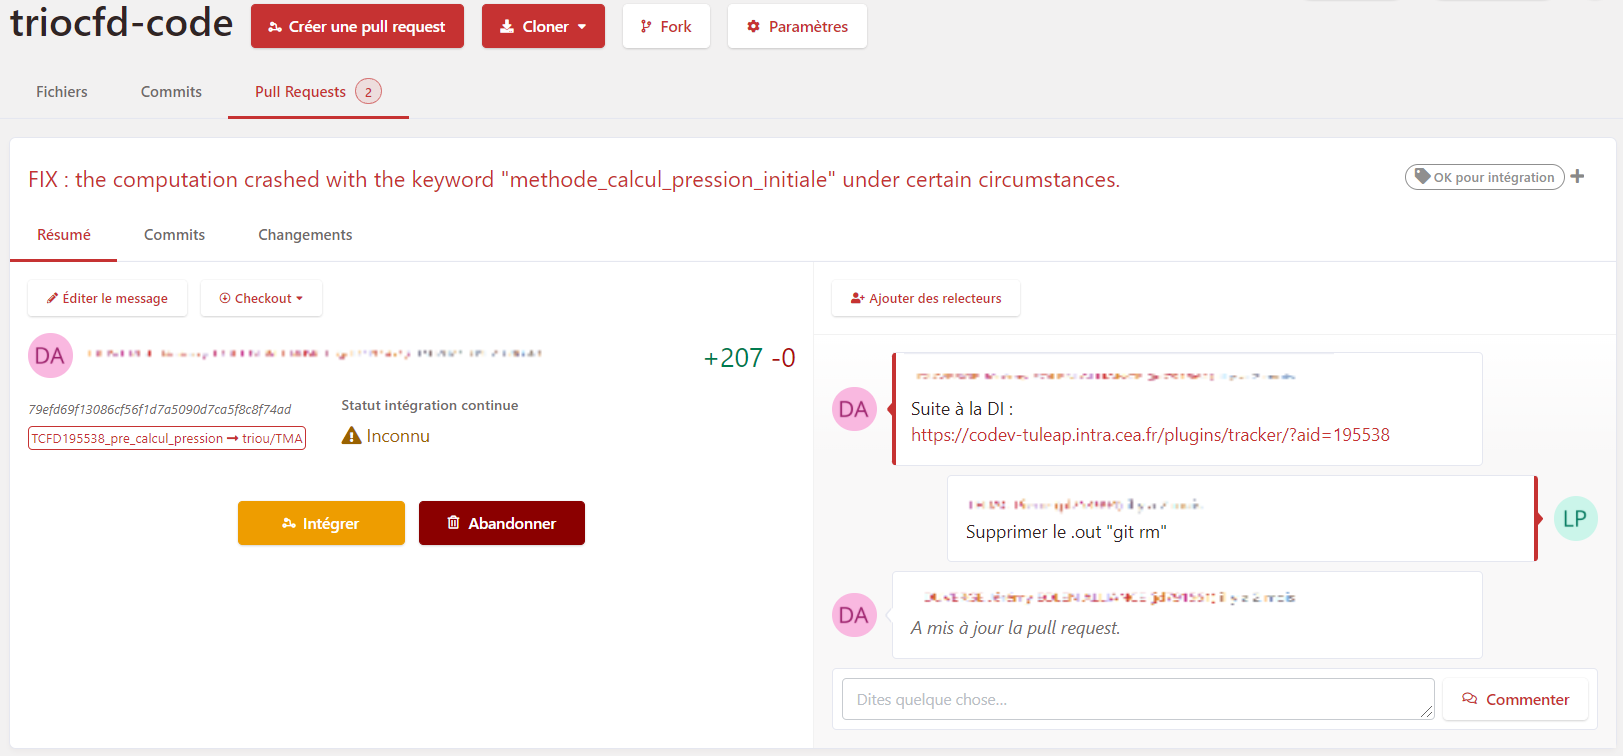
\includegraphics[width=16cm]{pictures/echangesRelecture.png}\vspace*{0.1cm}
   \captionof{figure}{\label{figure:relecture}Exemple d'échange lors de la relecture d'une branche}
\vspace*{0.7cm}   
Suite à la relecture, un commit supplémentaire pourra amené à être fait sur la branche du développement et la Pull Request, mise à jour.\\
Une 	fois la revue de code approuvée, le relecteur placera un tag \texttt{OK pour intégration} (voir figure \ref{figure:relecture} en haut à droite) signifiant que la branche du développement a passé avec succès cette étape et peut alors être intégrée dans le code.\\
L'intégrateur intervient alors en rapatriant 	la branche du développeur dans la branche de développement de TrioCFD (branche triou/TMA) à date. La branche de développement ayant pu recevoir d'autres intégrations depuis la création de la branche du développeur, il vérifie la bonne compilation du code sur la branche de développement avec les nouvelles fonctionnalités et lance la base de vérification. Si une de ces actions ne donnaient pas le résultat escompté, l'intégrateur corrigera la branche de développement avec, potentiellement, l'aide du développeur. Une fois ces 2  contrôles (compilation + vérification) atteints avec succès, la branche du développeur est commitée dans la branche triou/TMA et celle-ci est poussée sur le dépôt distant. Les tests de vérification quotidiens tourneront donc, le soir même, sur cette nouvelle version du code et le statut de la fiche Tuleap associée passera alors en état \texttt{MERGED} (voir figure \ref{figure:workflow_Trio}). La base de Validation sera lancée sur cette nouvelle version du code le week-end suivant et lorsque la non-régression sera atteinte, la fiche Tuleap associée sera fermée (statut \texttt{CLOSED}). L'ensemble du processus de développement sera alors achevé et l'action de développement sera considérée comme terminée.

%\chapter{Processus d'une \'etude}
%\lhead{Processus d'une \'etude}
%\rhead{METHODOLOGIES ET PROCEDURES}
%\vspace{1cm}
%\subsection{Sp\'ecification}\vspace{1cm}
%\subsection{R\'ealisation}\vspace{1cm}
%\subsection{Analyse et Synth\`ese}\vspace{1cm}
%\subsection{Validation}\vspace{1cm}
%\subsection{Archivage}\newpage


\chapter{\label{chapitre:livraison}Processus de Livraison}
\lhead{Processus de Livraison}
\rhead{METHODOLOGIES ET PROCEDURES}
La livraison est effectuée conjointement par l'équipe TMA et l'équipe CEA. Elle commence par la définition exacte de la date de sortie de version. 15 jours avant cette date, l'ensemble des branches (développements et correctifs) doivent avoir été intégrés dans la branche en développement (\texttt{triou/TMA}). D'autres intégrations mineures pourront éventuellement avoir lieu ensuite, notamment en cas d'échec de l'étape de validation de la non-régression. Les étapes importantes qui rythment la livraison sont décrites dans les sections suivantes.
\subsection{Étape 1 : Vérification et Validation de la non-r\'egression}
Une fois l'ensemble des correctifs et développements intégrés dans la version, la base de vérification tourne une dernière fois sur l'ensemble des machines du parc afin de s'assurer qu'il n'y ait aucune différence de comportement entre les différentes configurations couvertes. L'atelier de génie logiciel est alors désactivé jusqu'à la livraison de la version.\\
La base de validation est lancée une première fois et les non régressions vis à vis de la dernière exécution de la base de validation sont analysées afin de maîtriser les éventuels impacts des dernières intégrations (voir méthodologie décrite au chapitre \ref{chapitre:validation}). Elle est également lancée en prenant comme version de référence, la dernière version livrée du code. Les écarts obtenus correspondent à la concaténation de l'ensemble des différences identifiées lors du lancement hebdomadaire du processus de validation. Des jdds qui n'ont pas subi d'écarts lors des différentes validations intermédiaires ne doivent donc pas apparaître à ce moment-là.\\
Une fois ces 2 exécutions complètement analysées et justifiées, la nouvelle version du code est considérée comme validée. Les sources du code et les jdds ne devront plus être touchés jusqu'à ce que la livraison soit achevée.
\subsection{Étape 2 : Finalisation de la documentation et dernières intégrations}
L'étape suivante consiste, dans un premier temps, à mettre à jour toute la documentation afin notamment de faire évoluer le numéro de version, mais également de faire apparaître l'ensemble des évolutions qui ont eu lieu dans le code depuis la dernière livraison. Ceci concerne les documents cités au chapitre \ref{chapitre:doc-trio}. Une fois l'ensemble de la documentation mise à jour, celle-ci est intégrée dans la branche \texttt{triou/TMA} et constituera le dernier point de commit. La branche de développement de TrioCFD est alors mergée avec la branche \texttt{master} et un tag est apposé sur chacune de ces 2 branches avec le nom de la version livrée.
\subsection{Étape 3 : G\'en\'eration de l'archive et livraison via SourceForge/GitHub}
Vient ensuite l'étape de la mise à disposition aux utilisateurs et développeurs extérieurs au CEA. La nouvelle version leur est transmise via GITHUB depuis 2021 à l'adresse \url{https://github.com/cea-trust-platform/TrioCFD-code}. Auparavant, la plateforme utilisée était Sourceforge. La version est disponible sous GITHUB via 2 formats :
\begin{itemize}
   \item format archive : regroupe dans une archive l'ensemble du code source, des procédures ainsi qu'un pannel représentatif des fiches de validation du code. Cette archive doit être téléchargée et décompressée sur la machine où l'installation doit avoir lieu.
   \item format base git : contient l'ensemble du code, des jdds et des procédures de TrioCFD identique au dépôt GIT de TrioCFD hébergé sur Tuleap. La dernière version livrée correspondra à la branche \texttt{master} du dépôt GITHUB.
\end{itemize}
Pour les utilisateurs, il est recommandé de récupérer la version livrée sous le format archive, tandis que pour les développeurs, le dépôt GITHUB est à privilégier.
\subsection{Étape 4 : Mise \`a disposition sur les Clusters}
Finalement, la nouvelle version sera livrée aux utilisateurs CEA avec son installation sur l'ensemble des clusters répertoriés (5). Ils pourront également utiliser la version réseau de cette nouvelle version disponible sous \texttt{/home/triou}.\vspace{1cm}

A l'issue de toutes ces étapes, un mail sera envoyé à la communauté CEA de TrioCFD, décrivant les évolutions du code depuis la dernière version livrée et donnant les différents liens pour l'utiliser. Pour la communauté extérieure au CEA, l'information sera communiquée par le site de TrioCFD (voir chapitre \ref{chapitre:site}).\\
A l'issue de cette démarche, les intégrations reprendront dans le code en vue de l'enrichir pour la version suivante.

\chapter{Demande de maintenance}
\lhead{Demande de maintenance}
\rhead{METHODOLOGIES ET PROCEDURES}
Les actions de la TMA sur TrioCFD se font dans le cadre d'un cahier des charges relatif à la prestation de maintenance informatique des codes de calcul en thermohydraulique. Le contrat en cours est régi par le cahier des charges référencé : DES/ISAS/DM2S/STMF/DIR/ST/2021-66801/A. Celui-ci a débuté le 01/04/2021 pour une durée de deux ans avec la possibilité de le renouveler 3 fois pour une durée d'un an à chaque fois. Ce contrat est commun à différents codes du CEA.\\
Dans le cadre de ce contrat, diverses actions sur le code sont gérées par la TMA avec un suivi régulier de la part du CEA par le RLP et le Responsable de Code. Outre les échanges quotidiens, plusieurs réunions contractuelles doivent avoir lieu pour assurer le suivi :\\ 
\begin{itemize}[label=$\Rightarrow$, font=\LARGE]
   \item les \textbf{réunions de suivi hebdomadaires} qui permettent de faire un suivi rapproché des actions en cours, revoir les priorisations sur le code concerné en cas de besoins urgents des utilisateurs, ou échanger sur les difficultés rencontrées lors de la résolution des demandes de maintenance;
   \item les \textbf{COSUIV}, se déroulant de façon mensuel, permettent de faire le même suivi que les réunions hebdomadaires mais la priorisation est faite en regard des besoins de l'ensemble des codes à la charge de la TMA. Ainsi, si une échéance importante est prévue sur un code, les actions le concernant seront mises en priorité haute par rapport à celle des autres codes. Il se tient en présence du RPL, de l'ensemble des Responsables de Code et de l'ensemble de l'équipe TMA et donne lieu à compte-rendu de réunion rédigé par le RML.
   \item les \textbf{COPIL} ont lieu de fa\c con bi-mensuelle et réunit les chargés d'affaire (CEA et TMA), les RPL, les Responsables de Code, les RML (et éventuellement les Chefs de Laboratoires portant les codes et Chef de Service). Les COPIL permettent se s'assurer que les attendus contractuels sont bien respectés de part et d'autre. Un compte-rendu de réunion trace l'ensemble des constats fait lors du COPIL.
\end{itemize}

Les différentes actions à la charge de la TMA ainsi que leur méthodologie de traitement sont décrites dans ce chapitre.
\subsection{Prise en compte et analyse des demandes}
Toute question arrivant dans la boîte mail \href{mailto:trust@cea.fr}{trust@cea.fr} est prise en charge par la TMA avec un délai de traitement d'un jour ouvré. Après une première analyse, une fiche de Demande d'Intervention est créée par la TMA pour chaque problème rencontré. Cette étape préliminaire d'analyse permet de lui affecter de catégorie parmi celles détaillées ci-après. Lors du traitement de la Demande d'Intervention, si il s'avère que la catégorie n'a pas été correctement identifiée, elle pourra être mise à jour lors de son traitement.\\
La saisie sous forme de fiche de chacun des mails reçus permet de garantir un bon suivi des difficultés rencontrés et de garantir une réponse à l'ensemble des sollicitations   re\c cues.
\subsection{Traitement des Assistances Aux Utilisateurs (AAU)}
L'équipe de TMA est souvent sollicitée par les utilisateurs car un de leurs cas tests n'aboutit pas favorablement. La Demande d'Intervention est alors classée comme Assistance Aux Utilisateurs. A ce stade, rien ne garantit encore que l'erreur vienne effectivement d'un problème au niveau de la construction du jdd. Les travaux commenceront par la modification de plusieurs paramètres, bien connus pour jouer sur la stabilité des calculs comme le pas de temps, le facsec ou le solveur utilisé. Si ces premiers tests s'avèrent concluant et permettent d'arriver à une fin propre du calcul, cela voudra dire que le jdd envoyé nécessitait juste de jouer sur ces paramètres numériques. \\
En cas contraire, si le jdd fourni par l'Initiateur est complexe, on essayera de simplifier progressivement le jdd afin de mieux cerner l'élément problématique. Ce procédé de simplification couplé à l'analyse des messages obtenus dans le fichier de sortie (fichier .err) permettront de simplifier les travaux. Si le problème relève bien du jdd, l'équipe de TMA sera en mesure d'identifier rapidement le problème de modélisation que l'utilisateur aurait pu introduire dans ce jdd. La TMA proposera alors une version fonctionnelle du jdd à l'utilisateur en lui expliquant les modifications effectuées et la raison. Si l'utilisateur est satisfait de ces modifications, la DI passe en statut \texttt{Treated/Resolved} et les travaux sont considérés comme achevés.\\
Parfois, il s'avère que la TMA ne parvienne pas à résoudre le problème immédiatement car celui-ci ne provient pas du jdd en lui-même, mais relève d'un bug au niveau du code. La DI sera alors requalifiée dans la catégorie Maintenance Corrective.\\

Le contrat de TMA actuel prévoit 25 demandes Assistance Aux Utilisateurs par an sur TrioCFD.

\subsection{Traitement des Maintenances Correctives (MC)}
Pour rappel, une maintenance corrective est la correction d'anomalies dans les sources du code, dans les outils de maintenance, dans la documentation et dans les jeux de données de la base de test.\\
Une fois la fiche de Demande d'Intervention créée et identifiée dans cette catégorie, les travaux sont initiés sur le jdd fourni par l'Initiateur pour reproduire le problème constaté. Si le jdd fourni est complexe, celui-ci sera simplifié afin de mieux cerner l'élément source de bug dans le jdd. Une fois le problème reproduit sur un cas test élémentaire, les travaux de deboggage débuteront jusqu'à la bonne résolution du jdd fourni. Une fois cette étape atteinte en local, une branche GIT sera créée avec la même dénomination que décrite précédemment (voir la section \ref{subsec:WorkflowGIT}), c'est-à-dire avec le numéro de la DI correspondante sur le BugTracker, contentant l'ensemble des sources modifiées ainsi que le cas test ayant permis sa détection. Le Workflow présenté précédemment sera suivi, jusqu'à la clôture de la DI.\\

Le contrat de TMA actuel prévoit 5 demandes de Maintenance Corrective par an sur TrioCFD.

\subsection{Traitement des Maintenances Evolutives (ME)}
Toute intervention relevant de la maintenance évolutive sera précisément circonscrite, spécifiée et tracée et représentera au plus un volume de travail estimé à 10 h. jours (estimation validée par le CEA). Les interventions de maintenance évolutive demandant plus que 10 jours et moins de 20 jours de travail sont hors des prestations forfaitaires mais s'inscrivent dans le cadre des prestations sur devis. Les interventions de maintenance évolutive demandant plus de 20 jours de travail seront traitées dans un autre cadre que celui du contrat de TMA. Elles entrent également dans la partie forfaitaire du marché actuel.\\

Une Maintenance Évolutive correspond à une action légère de développement avec une répartition des actions décrites au Chapitre \ref{chapter:dev} de cette partie entre l'équipe CEA et l'équipe TMA. Ce type de Demande d'Intervention se fait par sollicitation du RPL vers l'équipe de TMA. Le RPL commence par créer une fiche de Demande d'Intervention dans le BugTracker TrioCFD. Il y précise, à l'aide l'Initiateur, les spécifications (voir section \ref{subsec:specif}) attendues dans le cadre de l'action.\\

Lors d'un COSUIV, l'action est détaillée par le RPL à l'équipe TMA (plusieurs rebouclages peuvent être faits afin de bien cerner l'action) puis le RML établit un chiffrage pour mener à bien la demande de Maintenance Évolutive. Suite à ce chiffrage, le RPL donne son accord (ou non) pour lancer l'action et précise dans la fiche du BugTracker, l'échéance attendue. Le responsable de l'action dans l'équipe TMA est alors en charge d'effectuer les étapes 2, 3 et 4 précisées dans le Chapitre \ref{chapter:dev} de cette partie, avec un point d'avancée à la fin de chacune avec le RPL. L'Initiateur peut également intervenir à l'étape 4 afin de s'assurer que le développement fournit bien les fonctionnalités et résultats attendus. L'étape 5 de relecture et d'intégration est à la charge du CEA. \\

Le contrat de TMA actuel prévoit 2 demandes de Maintenance Évolutive par an sur TrioCFD.

\subsection{Traitement des DI LIV}
L'équipe de TMA est en charge d'assurer 2 livraisons du code chaque année, généralement une fin juin et la seconde mi-décembre. Dans le cadre du marché actuel, il s'agit d'une action sur bordereau de prix (périmètre et chiffrage associé bien défini). Le CEA définit le planning et les destinataires des livraisons de ses logiciels dans les lettres de cadrage semestrielles. Un déplacement sur le site du client du CEA peut éventuellement être nécessaire. 
La livraison des nouvelles versions est planifi\'ee par le CEA, qui en confie une partie de la pr\'eparation et de l'ex\'ecution \`a l'\'equipe TMA (voir chapitre \ref{chapitre:livraison}).\\

Les t\^aches \`a accomplir comprennent notamment :
\begin{itemize}
    \item La compilation sur diff\'erents OS (une douzaine) ;
    \item Le passage des diff\'erents tests (non r\'egression, v\'erification, ...) ;
    \item La g\'en\'eration de la version, la mise à disposition sur l'outil de partage (GITHUB) et la création de l'archive ;
    \item La mise \`a jour d'une partie la documentation ; 
    \item L'\'etablissement de la note de version ;
    \item Les installations de la version pour chaque OS sur le r\'eseau interne du CEA et les calculateurs (3 \`a 4) du CCRT.
\end{itemize}


\subsection{Traitement des DI FOR}
Ce type de Demande d'Intervention correspond à la dispense de formation auprès des utilisateurs du code. Elles sont au nombre de 2 par an sur TrioCFD, généralement en Mars et en Octobre. Dans le cadre du marché actuel, il s'agit également d'une action sur bordereau de prix (périmètre et chiffrage associé bien défini). Elles ont lieu sur les sites CEA en région parisienne ou en province dans des locaux prévus à cet effet. La durée des sessions est variable, de 1 à 2 jours suivant les codes et les sujets traités. Le nombre de participants est aussi variable, au maximum 12 par session. Les formations peuvent être dispensées en Français ou en Anglais suivant la demande du CEA. Les formations sont planifiées et organisées par le CEA (présentation dans les lettres de cadrage semestrielles) qui en confie la préparation et l'exécution au titulaire du contrat de TMA. \\

Ce type d'activité est identifié comme DI dans le BugTracker à des fins d'organisation/planification de l'activité de maintenance. La fiche de BugTracker permet également d'assurer le suivi des personnes assistant à la formation. Les tâches incombant à la TMA comprennent la préparation des machines et logiciels de la salle de formation, la préparation/mise à jour des supports de formation et la dispense d'une partie des formations.\\

La formation dispensée sur TrioCFD est une formation à destination des utilisateurs avec, pour commencer, une phase de prise en main puis une description et une démonstration des capacités du code et également de nombreux exercices illustrant les différents domaines et utilisations possibles. Une seconde formation à destination des développeurs est supportée par l'équipe TRUST mais convient également parfaitement aux développeurs de TrioCFD puisque tous deux utilisent le même langage, la même architecture et la même philosophie de codage. Elle dure également 2 jours et nécessite la formation dite "utilisateur" comme pré-requis.\\

En terme de déroulé, le CEA et la TMA commencent par définir la date exacte pour la dispense de la formation, environ 2 mois avant les mois habituels, soit en janvier et en août. Une fois cette date définie, le RPL s'assure de réserver la salle de formation. Un mail d'annonce est  envoyé, dans la foulée, par la TMA aux utilisateurs répertoriés du projet. Toutes les réponses sont archivées dans la fiche correspondante du BugTracker. 1 mois avant la formation, les participants sont sélectionnés par date de réception de leur demande avec un ajustement possible en cas de besoin dûment justifié. La TMA les en informe en rappelant la date et le lieu exacte. 15 jours avant la formation, la TMA installe la dernière version de TRUST et de TrioCFD sur les machines sur lesquelles la formation sera dispensée et fournit les supports au CEA pour relecture et impression. 1 semaine avant la formation, la TMA envoie un dernier mail de rappel aux participants de la session. Durant la formation, l'équipe TMA est en charge de la présentation des supports et de l'encadrement des exercices avec un support de l'équipe CEA. En fin de formation, un questionnaire de satisfaction est fourni aux participants afin de faire évoluer leur contenu si besoin.








